\documentclass{article}

\usepackage[utf8]{inputenc}
\usepackage{xeCJK}
\usepackage{kotex}
\usepackage{minted}
\usepackage{mdframed}
\usepackage{ntheorem}
\usepackage{fontspec}
\usepackage{color}
\usepackage{graphicx}
\usepackage[a4paper, top=15mm, bottom=15mm, left=20mm, right=20mm]{geometry}

\definecolor{codeblockbackground}{RGB}{245, 245, 245}
\definecolor{codeblockborder}{RGB}{200, 200, 200}

\theoremstyle{nonumberplain}
\newmintedfile[javacode]{java}{
  linenos=true,
  breaklines,
  fontfamily=D2Coding,
  framesep=2mm,
  bgcolor=codeblockbackground
}
\newminted[console]{text}{
  breaklines,
  fontfamily=D2Coding,
  framesep=2mm,
  bgcolor=codeblockbackground
}
\newmdtheoremenv[%
  backgroundcolor=codeblockbackground,
  linecolor=codeblockborder,
  outerlinewidth=3
]{code}{}

\graphicspath{ {./tex/} }

\title{자바프로그래밍및실습 과제 3}
\author{214823 박종현}
\date{May 2022}

\begin{document}

\maketitle
\pagebreak



\section{과제 1}
\subsection{소스코드}

\javacode{java/Prob1/Average.java}

\subsection{실행 예제}
\subsubsection{예제 1}
\begin{console}
java Average.java 1 2 3 5 7 8 1 2 3 4
입력받은 인자 값의 평균은 : 3.6
\end{console}
\makebox{
  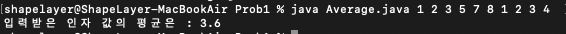
\includegraphics[width=\linewidth]{Prob1}
}
\subsubsection{예제 2}
\begin{console}
java Average.java 1 2 3 4 5 6 7 8 9 10          
입력받은 인자 값의 평균은 : 5.5
\end{console}



\section{과제 2}
\subsection{소스코드}
\javacode{java/Prob2.java}

\subsection{실행 예제}
\subsubsection{예제 1}
\begin{console}
java Prob2.java
과목 이름 >> Jaba
없는 과목입니다.
과목 이름 >> Java
Java의 점수는 95
과목 이름 >> 안드로이드
안드로이드의 점수는 55
과목 이름 >> 그만
\end{console}
\makebox{
  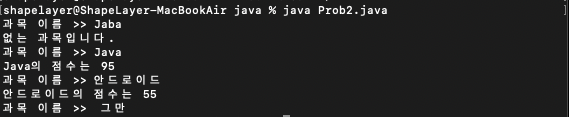
\includegraphics[width=\linewidth]{Prob2}
}
\subsubsection{예제 2}
\begin{console}
java Prob2.java
과목 이름 >> HTML5
HTML5의 점수는 76
과목 이름 >> html5
html5의 점수는 76
과목 이름 >> 그만
\end{console}



\section{과제 3}
\subsection{소스코드}
\javacode{java/Prob3.java}

\subsection{실행 예제}
\subsubsection{예제 1}
\begin{console}
java Prob3.java
곱하고자 하는 두수 입력>>2.5 4
실수는 입력하면 안됩니다.
곱하고자 하는 두수 입력>>4 3.5
실수는 입력하면 안됩니다.
곱하고자 하는 두수 입력>>4 3
4x3=12
\end{console}
\makebox{
  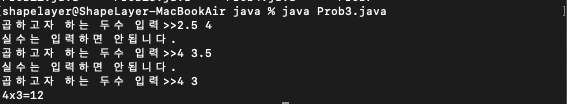
\includegraphics[width=\linewidth]{Prob3}
}
\subsubsection{예제 2}
문제에서 제시하지 않은 조건: 채점 대상 아님
\begin{enumerate}
  \item InputMismatchException은 제시한 입력 타입과 맞지 않으면 발생: String형도 Integer가 아니므로 "실수는 입력하면 안됩니다." 출력됨
  \item 문제 제시 코드에서 변수 타입을 Integer로 설정하였으므로, 연산 결과가 Integer 범위를 초과하면 잘못된 값이 출력됨
\end{enumerate}
\begin{console}
java Prob3.java
곱하고자 하는 두수 입력>> 문자열입력 문자열입력
실수는 입력하면 안됩니다.
곱하고자 하는 두수 입력>>10000000 10000000
10000000x10000000=276447232
\end{console}



\section{과제 4}
\subsection{소스코드}
\javacode{java/Prob4.java}
\subsection{실행 예제}
\subsubsection{예제 1}
\begin{console}
java Prob4.java
컴퓨터와 가위 바위 보 게임을 합니다.
가위 바위 보! >> 바위
사용자 = 바위, 컴퓨터 가위, 사용자가 이겼습니다.
가위 바위 보! >> 가위
사용자 = 가위, 컴퓨터 보, 사용자가 이겼습니다.
가위 바위 보! >> 그만
게임을 종료합니다.
\end{console}
\makebox{
  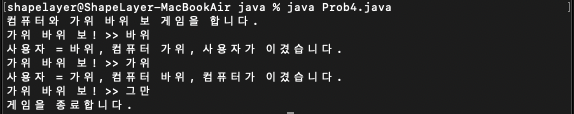
\includegraphics[width=\linewidth]{Prob4}
}



\section{과제 5}
\subsection{소스코드}
\javacode{java/Prob5.java}
\subsection{실행 예제}
\subsubsection{예제 1}
\begin{console}
java Prob5.java
LG에서 만든 2017년형 32인치 TV
\end{console}
\makebox{
  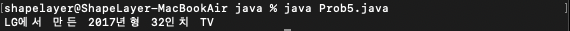
\includegraphics[width=\linewidth]{Prob5}
}



\section{과제 6}
\subsection{소스코드}
\javacode{java/Prob6.java}
\subsection{실행 예제}
\subsubsection{예제 1}
\begin{console}
java Prob6.java
수학, 과학, 영어순으로 3개의 점수 입력>>90 88 96
평균은 91
\end{console}
\makebox{
  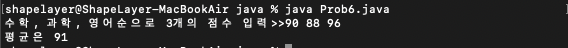
\includegraphics[width=\linewidth]{Prob6}
}
\subsubsection{예제 2}
\begin{console}
java Prob6.java
수학, 과학, 영어순으로 3개의 점수 입력>>85 90 95
평균은 90
\end{console}



\section{과제 7}
\subsection{소스코드}
\javacode{java/Prob7/Phonebook.java}
\subsection{실행 예제}
\subsubsection{예제 1}
\begin{console}
java Phonebook.java
인원수 >> 3
이름과 전화번호 (이름과 번호는 빈 칸없이 입력)>> 황기태 777-7777
이름과 전화번호 (이름과 번호는 빈 칸없이 입력)>> 나명품 999-7777
이름과 전화번호 (이름과 번호는 빈 칸없이 입력)>> 최자바 333-1234
저장되었습니다…
검색할 이름 >> 황기순
황기순 이(가) 없습니다.
검색할 이름 >> 최자바
최자바의 번호는 333-1234입니다.
검색할 이름 >> 그만
프로그램을 종료합니다.
\end{console}
\makebox{
  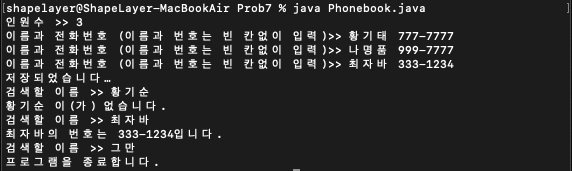
\includegraphics[width=\linewidth]{Prob7}
}



\section{과제 8}
\subsection{소스코드}
\javacode{java/Prob8/StaticEx.java}
\subsection{실행 예제}
\subsubsection{예제 1}
\begin{console}
java StaticEx.java
[ 1 5 7 9 3 6 -1 100 77 ]
\end{console}
\makebox{
  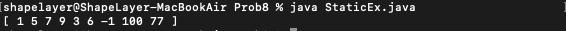
\includegraphics[width=\linewidth]{Prob8}
}



\section{과제 9}
\subsection{소스코드}
\javacode{java/Prob9/DicApp.java}
\subsection{실행 예제}
\subsubsection{예제 1}
\begin{console}
java DicApp.java
한영 단어 검색 프로그램입니다.
한글 단어? 희망
희망은 hope
한글 단어? 아가
아가는 저의 사전에 없습니다.
한글 단어? 미래
미래는 future
한글 단어? 종료
프로그램을 종료합니다.
\end{console}
\makebox{
  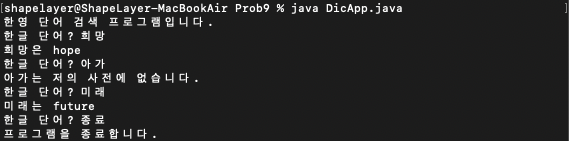
\includegraphics[width=\linewidth]{Prob9}
}
\subsubsection{예제 2}
\begin{console}
java DicApp.java
한영 단어 검색 프로그램입니다.
한글 단어? 사랑
사랑은 love
한글 단어? 아기
아기는 baby
한글 단어? 돈
돈은 money
한글 단어? 미래
미래는 future
한글 단어? 희망
희망은 hope
한글 단어? 종료
프로그램을 종료합니다.
\end{console}



\section{과제 10}
\subsection{소스코드}
\javacode{java/Prob10.java}
\subsection{실행 예제}
\subsubsection{예제 1}
\begin{console}
java Prob10.java
32인치 1024컬러
\end{console}
\makebox{
  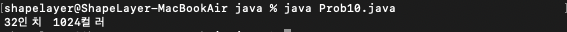
\includegraphics[width=\linewidth]{Prob10}
}



\section{과제 11}
\subsection{소스코드}
\javacode{java/Prob11.java}
\subsection{실행 예제}
\subsubsection{예제 1}
\begin{console}
java Prob11.java
나의 IPTV는 192.1.1.2 주소의 32인치 2048컬러
\end{console}
\makebox{
  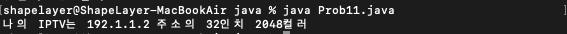
\includegraphics[width=\linewidth]{Prob11}
}



\section{과제 12}
\subsection{소스코드}
\javacode{java/Prob12.java}
\subsection{실행 예제}
\subsubsection{예제 1}
\begin{console}
java Prob12.java
BLACK색의 (0, 0)의 점입니다.
RED색의 (5, 5)의 점입니다.
\end{console}
\makebox{
  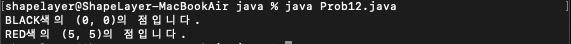
\includegraphics[width=\linewidth]{Prob12}
}



\section{과제 13}
\subsection{소스코드}
\javacode{java/Prob13.java}
\subsection{실행 예제}
\subsubsection{예제 1}
\begin{console}
java Prob13.java
(1, 2, 3)의 점입니다.
(1, 2, 4)의 점입니다.
(10, 10, 3)의 점입니다.
(100, 200, 300)의 점입니다.
\end{console}
\makebox{
  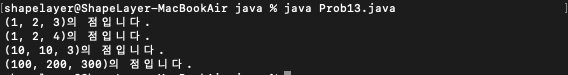
\includegraphics[width=\linewidth]{Prob13}
}



\end{document}
